\def\Lun{4}
\def\Ldeux{\Lun/3}
\def\Ltrois{\Ldeux/3}
\begin{tikzpicture}
	\draw[black] (0,0) -- (0:\Lun);
\end{tikzpicture}
\begin{tikzpicture}
	\draw[red] (0,0) --++ (0:\Ldeux) --++ (60:\Ldeux) --++ (-60:\Ldeux) --++ (0:\Ldeux);
\end{tikzpicture}
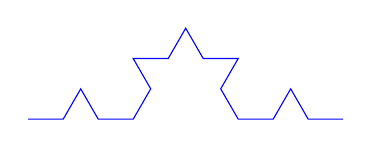
\begin{tikzpicture}
	\draw[blue] (0,0)
		--++ (0:\Ltrois) --++ (60:\Ltrois) --++ (-60:\Ltrois) --++ (0:\Ltrois)
		--++ (60:\Ltrois) --++ (120:\Ltrois) --++ (0:\Ltrois) --++ (60:\Ltrois)
		--++ (-60:\Ltrois) --++ (0:\Ltrois) --++ (-120:\Ltrois) --++ (-60:\Ltrois)
		--++ (0:\Ltrois) --++ (60:\Ltrois) --++ (-60:\Ltrois) --++ (0:\Ltrois);
\end{tikzpicture}